\documentclass[tikz,border=5pt]{standalone}
\usepackage{amsmath,amssymb,fontspec,unicode-math}
\setmainfont{STIXTwoText-Regular.otf}
\setmathfont{STIXTwoMath-Regular.otf}
\usetikzlibrary{positioning,arrows.meta,calc,decorations.pathreplacing}
\definecolor{hmtgray}{gray}{0.3}
\definecolor{hmtblue}{gray}{0.15}
\definecolor{hmtgold}{gray}{0.3}
\definecolor{hmtgreen}{gray}{0.1}
\definecolor{hmtred}{gray}{0.25}
\definecolor{hmtlightblue}{gray}{0.92}
\definecolor{hmtlightgold}{gray}{0.83}
\definecolor{hmtlightgreen}{gray}{0.97}
\definecolor{hmtlightred}{gray}{0.73}
\begin{document}
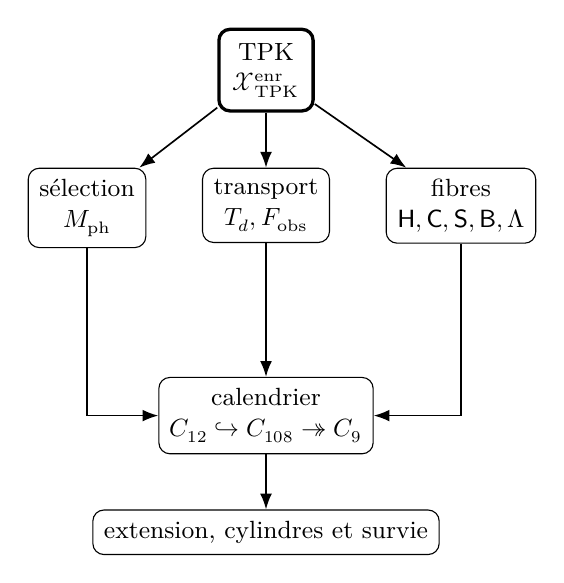
\begin{tikzpicture}[
  node distance=7mm and 9mm,
  every node/.style={font=\small,align=center},
  root/.style={draw=black,very thick,rounded corners,inner sep=5pt},
  op/.style={draw=black,rounded corners,inner sep=4pt},
  edge/.style={-{Latex[length=2mm]},semithick}
 ]
  \node[root] (tpk) {TPK\\$\mathcal X_{\rm TPK}^{\rm enr}$};
  \node[op,below left=of tpk] (sel) {sélection\\$M_{\rm ph}$};
  \node[op,below=of tpk] (mov) {transport\\$T_d,F_{\rm obs}$};
  \node[op,below right=of tpk] (fib) {fibres\\$\mathsf H,\mathsf C,\mathsf S,
    \mathsf B,\Lambda$};
  \node[op,below=17mm of mov] (cal) {calendrier\\$C_{12}\hookrightarrow
    C_{108}\twoheadrightarrow C_9$};
  \node[op,below=of cal] (ext) {extension, cylindres et survie};
  \draw[edge] (tpk) -- (sel);
  \draw[edge] (tpk) -- (mov);
  \draw[edge] (tpk) -- (fib);
  \draw[edge] (sel) |- (cal);
  \draw[edge] (mov) -- (cal);
  \draw[edge] (fib) |- (cal);
  \draw[edge] (cal) -- (ext);
 \end{tikzpicture}
\end{document}

